\documentclass[11pt]{article}

\usepackage[letterpaper,margin=1in]{geometry}
\usepackage[utf8]{inputenc}
\usepackage[T1]{fontenc}
\PassOptionsToPackage{hyphens}{url}
\usepackage{url}
\usepackage{hyperref}
\usepackage{booktabs}
\usepackage{amsfonts}
\usepackage{amsmath}
\usepackage{xcolor}
\usepackage{graphicx}
\usepackage{multirow}
\setlength{\parskip}{0.3ex}
\hypersetup{colorlinks=true, linkcolor=blue!50!black, urlcolor=blue!50!black, citecolor=blue!50!black, breaklinks=true}
% Allow URL line breaks at slashes, dashes, and dots
\def\UrlBreaks{\do\/\do-\do.\do\_}

\title{\vspace{-2em}Simplified Quantization for Edge-Ready Language Models:\\
Salience-Guided Mixed-Precision Post-Training Quantization at 1.61~Bits}

\author{Anshul Dani \\ \small A20580060 \\ \small \texttt{adani2@hawk.illinoistech.edu} \and
        Rohit Lahori \\ \small A20582911 \\ \small \texttt{rlahori@hawk.illinoistech.edu}}
\date{Illinois Institute of Technology --- CS595-2 --- May 2026}

\begin{document}

\maketitle
\vspace{-0.5em}

\begin{abstract}
\small
Large language models are too large for edge devices, and uniform post-training
quantization (PTQ) below 2~bits/weight collapses model accuracy.
We present \textbf{Salient-Quant} (SMQ), a three-phase PTQ framework that
allocates a mixed $\{1,2,4\}$-bit budget across weights according to a
five-metric salience ensemble (magnitude L1/L2, gradient, Hessian-diagonal Fisher,
activation-aware scaling), and applies row-coherent block-wise quantization with
closed-form OLS scale refinement.
On \textbf{GPT-2 medium (345M)}, SMQ achieves WikiText-2 PPL of \textbf{541.05} at 1.61~bits/weight ---
$\mathbf{2{,}683\times}$ better than Uniform INT2 (1.45M PPL) at higher compression ($9.94\times$ vs.\ $7.97\times$).
On \textbf{LLaMA-3.2-1B}, SMQ reaches \textbf{35{,}831} PPL at 1.61~bits ($10.4\times$ compression) ---
$4.6\times$ better than Uniform INT2 and $2.8\times$ better than BitNet at the same scale.
A six-axis ablation study isolates each design choice, surfacing three findings that contradict
the project's design assumptions: (i)~magnitude alone is the strongest single salience signal,
(ii)~symmetric 2-bit beats asymmetric on LLaMA-1B by $9.6\times$, and (iii)~the dominant
accuracy lever is \emph{spatial coherence} of block-wise scales --- a row-wise quantization
fix alone took GPT-2 medium PPL from 12{,}173 to 541 ($22\times$), eclipsing every salience
metric.
We also document the seven engineering fixes needed to fit the pipeline within a 16~GB
Colab T4.
\end{abstract}

% =================================================================
\section{Motivation and Problem Statement}
\label{sec:intro}
% =================================================================

State-of-the-art LLMs require gigabytes of memory: LLaMA-3.2-1B at FP16 occupies 2.5~GB,
a 7B model needs $>$13~GB.
Edge devices typically expose under 256~MB of usable RAM, so deployment requires
$10\times$ or greater compression.
Post-training quantization (PTQ) is the preferred mechanism --- no fine-tuning, generalizes
across model families --- but sub-2-bit PTQ is brittle.
Uniform INT2 inflates GPT-2 medium WikiText-2 perplexity from 21.64 to $1.45\times 10^6$
(a $67{,}000\times$ degradation); BitNet's ternary scheme is no better as a PTQ
($1.56\times 10^6$ PPL) because it was designed for training-time integration.
The 4-bit regime (GPTQ, AWQ) is well-studied but only delivers $4\times$ compression.
The interesting 2-bit regime is where uniform methods break.

\textbf{This project asks:} can a non-uniform allocation of $\{1,2,4\}$ bits, guided by a
per-weight importance score, achieve a sub-2-bit average while preserving usable accuracy?
The answer addresses both an algorithmic question (what does ``important'' mean for weights?)
and a systems question (can the resulting pipeline fit and run within a commodity 16~GB GPU?).

\textbf{Contributions.}
(i)~A vectorized 5-metric salience ensemble computed in a single calibration pass.
(ii)~A greedy bit allocator that distributes $\{1,2,4\}$-bit budgets across all parameters
in a single \texttt{torch.topk} call (0.45~s for 345M weights).
(iii)~A row-coherent block-wise quantizer with closed-form OLS scale refinement, achieving
\textbf{541~PPL} at 1.61~bits on GPT-2 medium.
(iv)~A six-axis ablation study on LLaMA-3.2-1B with full JSON outputs released.
(v)~Documented engineering: seven memory and numerical-stability fixes that enabled the
pipeline to run on a 16~GB T4, including a row-coherence fix that alone gave $22\times$ PPL.

% =================================================================
\section{Background and Related Work}
\label{sec:related}
% =================================================================

\textbf{Uniform PTQ.} GPTQ~\cite{frantar2023gptq} quantizes LLMs to 4-bit via Hessian-based
optimal rounding; AWQ~\cite{lin2024awq} protects salient \emph{channels} at higher precision;
ZeroQuant~\cite{yao2022zeroquant} adds hardware-aware kernels.
All target 4-bit; none cross the 2-bit barrier.
\textbf{Sub-2-bit.} BitNet~\cite{wang2023bitnet} uses ternary weights at 1.58~bits but
requires training-time integration, collapsing as PTQ.
LLM.int8()~\cite{dettmers2022llm} mixes INT8/FP16 outliers but stops at 8-bit.
\textbf{Salience-aware.} SmoothQuant~\cite{xiao2023smoothquant} transfers difficulty
between activations and weights;
OBD~\cite{lecun1990obd} and OBS~\cite{hassibi1993obs} use Hessian information for pruning.
We extend this line by combining five complementary metrics into a per-weight ensemble used
for \emph{bit allocation} rather than pruning.
\textbf{Datasets and tools.} Calibration: C4 validation~\cite{raffel2020t5}.
Evaluation: WikiText-2~\cite{merity2017wikitext} and Penn Treebank.
Models: GPT-2~\cite{radford2019gpt2}, LLaMA-3.2-1B~\cite{touvron2023llama}.
Implementation: PyTorch 2.x, HuggingFace Transformers, Colab T4.

% =================================================================
\section{Methodology}
\label{sec:method}
% =================================================================

SMQ runs three sequential phases on a pre-trained model with access to a small calibration
set; no gradient updates are applied to model parameters.

\textbf{Phase 1 -- Salience scoring.}
Each weight gets a score from five min-max-normalized-per-layer metrics combined as
$s_{\text{ens}}(w) = \alpha_1 \hat{s}_{\text{L1}} + \alpha_2 \hat{s}_{\text{L2}}
+ \alpha_3 \hat{s}_{\text{grad}} + \alpha_4 \hat{s}_{\text{H}} + \alpha_5 \hat{s}_{\text{act}}$.
The metrics are
$s_{\text{L1}} = |w|$,
$s_{\text{L2}} = w^2$,
$s_{\text{grad}} = |w \cdot \nabla_w \mathcal{L}|$~\cite{lecun1990obd},
$s_{\text{H}} = \mathbb{E}[(\nabla_w \mathcal{L})^2]$ (empirical Fisher
diagonal~\cite{hassibi1993obs}),
and $s_{\text{act}}(w_{ij}) = |w_{ij}| \cdot \text{std}(x_j)$ following SmoothQuant.
Default $\boldsymbol{\alpha} = (0.15, 0.15, 0.25, 0.25, 0.20)$;
Section~\ref{sec:ablations} shows magnitude-heavy weighting empirically dominates at 1.61~b
on LLaMA-3.2-1B.

\textbf{Phase 2 -- Greedy bit allocation.}
Given $B_{\text{target}} = 1.61$ and bit choices $\mathcal{B} = \{1, 2, 4\}$:
initialize $b_i = 1$ for all weights, set $\text{budget} = (B_{\text{target}} - 1) \cdot N$,
then for each $b \in \{2, 4\}$ ascending, take the top-$k$ weights by salience
($k = \lfloor\text{budget}/(b{-}1)\rfloor$) and upgrade them to $b$ bits, decrementing the
budget.
The top-$k$ step is one GPU \texttt{torch.topk} call over all weights concatenated;
allocation completes in 0.45~s for 85M-quantizable-weight GPT-2 medium.

\textbf{Phase 3 -- Row-coherent mixed-precision quantization.}
Each weight is quantized at its assigned bit-width:
1-bit uses $q = \text{sign}(w) \cdot \overline{|w|}$ per block (BitNet-style);
2-bit uses 4 symmetric levels $\{\pm 0.5s, \pm 1.5s\}$;
4-bit uses INT4 symmetric (15 levels).
For 2- and 4-bit, given fixed level codes $\mathbf{L}$, the closed-form scale minimizing
$\|\mathbf{W} - s\mathbf{L}\|_2^2$ is $s^* = (\mathbf{W}\cdot\mathbf{L})/(\mathbf{L}\cdot\mathbf{L})$,
replacing a per-block Adam loop with two vectorized dot products.

\textit{The row-coherence fix.}
Our first implementation flattened each weight matrix into a 1D array before applying the
boolean salience mask, so block boundaries cut across unrelated rows --- the per-block scale
mixed weights from independent neurons, corrupting the OLS estimate.
Processing each row independently keeps blocks spatially coherent.
This single change reduced GPT-2 medium PPL from \textbf{12{,}173} to \textbf{541}
($22\times$); we revisit its outsized impact in Section~\ref{sec:bottleneck}.

% =================================================================
\section{Experimental Setup}
\label{sec:setup}
% =================================================================

\textbf{Hardware:} single Google Colab T4 GPU (16~GB VRAM, 14.56~GB usable),
$\sim$12.7~GB system RAM.
The T4 budget was the binding constraint that shaped seven implementation choices
(Section~\ref{sec:bottleneck}).
\textbf{Software:} Python 3.10, PyTorch 2.x, HuggingFace Transformers/datasets/hub.
Random seeds fixed.
\textbf{Models:}
GPT-2 small (124M, validation), GPT-2 medium (345M, primary GPT-2 evaluation), LLaMA-3.2-1B
(modern LLaMA evaluation; ablation target).
\textbf{Calibration:} GPT-2 uses $N{=}512$ samples at sequence length 512.
LLaMA uses $N{=}128{-}256$ at sequence length 256, batch size 1, due to T4 memory pressure
(Ablation~4 confirms $N{=}256$ is optimal on the 1B model).
\textbf{Baselines:} FP16 (uncompressed upper bound), Uniform INT2 (symmetric 2-bit
block-wise, block~64), BitNet ternary ($\{-1, 0, +1\} \times \overline{|W|}$ as PTQ),
Salient-Quant at 1.61~b.
GPTQ was disabled because the \texttt{auto-gptq} install repeatedly failed on Colab T4.
\textbf{Metrics:} perplexity on WikiText-2 raw test and Penn Treebank (sliding window,
stride~512, max length~1024); compressed model size ($\sum_\ell N_\ell b_\ell / 8$~bytes);
per-phase wall-clock; peak VRAM.
MMLU 5-shot and end-to-end inference latency were planned but deferred
(Section~\ref{sec:limits}).

% =================================================================
\section{Results and Analysis}
\label{sec:results}
% =================================================================

Table~\ref{tab:main} reports the main comparison on both models.
SMQ at 1.61~b is the only sub-2-bit method that does not collapse below uniform INT2.

\begin{table}[h]
\centering
\small
\caption{Main results on GPT-2 medium (345M) and LLaMA-3.2-1B.
PPL is on WT2 / PTB test sets (lower is better); Size is parameter footprint in GB.
$\dagger$ = our method.}
\label{tab:main}\label{tab:gpt2_main}\label{tab:llama_main}
\setlength{\tabcolsep}{6pt}
\renewcommand{\arraystretch}{1.05}
\begin{tabular}{@{}lc rrr c rrr@{}}
\toprule
& & \multicolumn{3}{c}{\textbf{GPT-2 medium (345M)}} & & \multicolumn{3}{c}{\textbf{LLaMA-3.2-1B}} \\
\cmidrule(lr){3-5}\cmidrule(lr){7-9}
Method & Bits & WT2 PPL$\downarrow$ & PTB PPL$\downarrow$ & Size (GB) & Bits & WT2 PPL$\downarrow$ & PTB PPL$\downarrow$ & Size (GB) \\
\midrule
FP16             & 16.0  & 21.64       & 22.53       & 0.61 & 16.0  & 10.96     & 11.32      & 2.47 \\
Uniform INT2     &  2.0  & 1{,}451{,}721 & 1{,}310{,}861 & 0.08 &  2.0  & 164{,}165 & 168{,}767  & 0.31 \\
BitNet ternary   &  1.0  & 1{,}556{,}522 & 1{,}448{,}814 & 0.04 &  1.58 & 99{,}786  & 104{,}487  & 0.16 \\
\midrule
\textbf{SMQ$^\dagger$} & \textbf{1.61} & \textbf{541.05} & \textbf{547.75} & \textbf{0.06}
                       & \textbf{1.61} & \textbf{35{,}831} & \textbf{31{,}859} & \textbf{0.24} \\
\bottomrule
\end{tabular}
\end{table}

\textbf{GPT-2 medium.}
SMQ is $\mathbf{2{,}683\times}$ better than Uniform INT2 on WT2 \emph{while using less
memory} (0.06 vs.\ 0.08~GB at 1.61 vs.\ 2.0 bits), and $2{,}874\times$ better than BitNet
at the same compression class.
The 541~PPL absolute number is still far from the 21.64 FP16 ceiling --- expected for
sub-2-bit PTQ without quantization-aware fine-tuning --- but the \emph{relative}
result shows salience-guided allocation rescues the model from catastrophic collapse.

\textbf{LLaMA-3.2-1B.}
SMQ is $\mathbf{4.6\times}$ better than Uniform INT2 and $2.8\times$ better than BitNet
at the same compression.
The absolute LLaMA PPL (35{,}831 vs.\ 10.96 FP16) is high: the 1B model's response to
sub-2-bit PTQ is more brittle than 345M's, consistent with the literature.
The bit-budget Pareto sweep (Appendix~\ref{app:bitbudget}) shows 1.61~b is the empirical
optimum among seven settings tested; targets $\geq 2.0$~b silently collapse to uniform
INT2 due to a known 4-bit-tier activation bug (Section~\ref{sec:limits}).

\textit{Reconciling Table~\ref{tab:main} with the ablations.}
The headline numbers above (541 on GPT-2~medium, 35{,}831 on LLaMA-1B) reflect the
deployed YAML configurations.
The ablation grids in Section~\ref{sec:ablations} sweep one axis at a time over the
post-OOM-fix pipeline, which differs from the deployed config along several axes
(\texttt{block\_size}, ensemble weighting, and on LLaMA the \texttt{asymmetric}
$\rightarrow$ \texttt{symmetric} choice surfaced in Ablation~6).
Absolute PPL across ablation rows is therefore \emph{not} directly comparable to
Table~\ref{tab:main}; the comparable quantity is the \emph{relative} ranking within
each ablation table.
On LLaMA, Ablation~6 specifically indicates that switching the deployed
\texttt{llama\_full.yaml} from \texttt{asymmetric} to \texttt{symmetric} should pull the
35{,}831 number toward the $\sim$30{,}800 seen at the same bit budget in
Table~\ref{tab:abl_llama}.

% =================================================================
\section{Ablation Studies}
\label{sec:ablations}
% =================================================================

We isolate six design choices.
Salience-metric and granularity ablations use GPT-2 medium where the row-coherence fix is
established; the rest use LLaMA-3.2-1B at 1.61~b with $N{=}256$ calibration samples.
\emph{Note on absolute values:} the ablation pipeline is a post-OOM-fix configuration that
differs from the deployed Table~\ref{tab:main} runs along several axes (block size,
ensemble weighting, scheme); compare \emph{within} an ablation table rather than
\emph{between} the ablations and the main results.

\textbf{Ablation 1 -- Salience metric (GPT-2 medium).}
Table~\ref{tab:abl_metric} compares each of the five metrics individually against the
ensemble.
The ensemble dominates every single metric;
\emph{magnitude} (L1/L2) is the strongest single predictor, contradicting the literature's
emphasis on gradient/Hessian sensitivity --- a useful finding for low-cost pipelines that
cannot afford a backward pass.
Hessian-only allocation breaks budget control: per-element Fisher scores are near-uniform,
so the allocator cannot rank weights and over-shoots to 2.0~b on average.

\textbf{Ablation 2 -- Granularity (GPT-2 medium).}
Per-element bit allocation is essential: coarsening to channel-wise costs $154\times$ in
PPL, layer-wise $291\times$.
The same pattern replicates on LLaMA (Ablation~5 below): coarse granularities also
\emph{undershoot} the bit budget (channel hits 1.54, layer 1.45) because group-level
allocation cannot fine-tune to 1.61.

\begin{table}[h]
\small
\centering
\begin{minipage}[t]{0.46\linewidth}
\centering
\caption{Ablation~1 (GPT-2 medium, 1.61~b).}
\label{tab:abl_metric}
\begin{tabular}{@{}lcc@{}}
\toprule
Metric & PPL$\downarrow$ & vs.\ Ensemble \\
\midrule
Magnitude L1 & 9{,}274  & $1.68\times$ \\
Magnitude L2 & 9{,}095  & $1.65\times$ \\
Gradient     & 72{,}671 & $13.2\times$ \\
Activation   & 27{,}128 & $4.92\times$ \\
Hessian (over-allocates)& 243{,}575 & $44\times$ \\
\midrule
\textbf{Ensemble} & \textbf{5{,}512} & --- \\
\bottomrule
\end{tabular}
\end{minipage}\hfill%
\begin{minipage}[t]{0.50\linewidth}
\centering
\caption{Ablation~2 (GPT-2 med) and Ablation~5 (LLaMA-1B).
Both at 1.61~b target.}
\label{tab:abl_gran}
\begin{tabular}{@{}lcc@{}}
\toprule
Granularity & GPT-2 PPL & LLaMA PPL (achieved bits) \\
\midrule
\textbf{Weight}  & \textbf{5{,}681} & \textbf{29{,}877} (1.60) \\
Channel & 872{,}569 & 228{,}927 (1.54) \\
Layer   & 1{,}654{,}710 & 190{,}060 (1.45) \\
\bottomrule
\end{tabular}
\end{minipage}
\end{table}

\textbf{Ablations 3, 4, 6, 7 -- LLaMA-3.2-1B sweeps.}
Table~\ref{tab:abl_llama} consolidates the four LLaMA-1B ablations at the 1.61~b target.
Each row varies one axis with all others held at default.

\begin{table}[!ht]
\footnotesize
\centering
\setlength{\tabcolsep}{5pt}
\renewcommand{\arraystretch}{0.95}
\caption{LLaMA-3.2-1B ablations (target 1.61~b, $N{=}256$, \texttt{block\_size}=32).
Achieved bits in parentheses.}
\label{tab:abl_llama}
\begin{tabular}{@{}llc@{}}
\toprule
Axis & Configuration & WT2 PPL$\downarrow$ \\
\midrule
\multirow{4}{*}{Ablation 3 -- Bit-budget sweep}
  & target~1.0~b   & 90{,}337 (1.00) \\
  & target~1.3~b   & 43{,}288 (1.28) \\
  & \textbf{target~1.61~b} & \textbf{29{,}721} (1.60) \\
  & target~$\geq$2.0~b (4 settings collapse to INT2) & 113{,}582 (2.00) \\
\midrule
\multirow{4}{*}{Ablation 4 -- Calibration size}
  & $N{=}128$  & 31{,}425 \\
  & \textbf{$N{=}256$}  & \textbf{29{,}877} \\
  & $N{=}512$  & 30{,}936 \\
  & $N{=}1024$ & 31{,}774 \\
\midrule
\multirow{2}{*}{Ablation 6 -- Quant scheme}
  & \textbf{Symmetric}  & \textbf{30{,}792} \\
  & Asymmetric (deployed in YAML) & 295{,}858 \\
\midrule
\multirow{5}{*}{Ablation 7 -- Ensemble weights $\boldsymbol{\alpha}$}
  & \textbf{Magnitude-heavy} (0.30, 0.30, 0.15, 0.15, 0.10) & \textbf{21{,}977} \\
  & Default (0.15, 0.15, 0.25, 0.25, 0.20) & 30{,}896 \\
  & Activation-heavy (0.10, 0.10, 0.15, 0.15, 0.50) & 34{,}803 \\
  & Uniform (0.20$\times$5)                            & 34{,}779 \\
  & Gradient-heavy (0.10, 0.10, 0.40, 0.30, 0.10)      & 49{,}095 \\
\bottomrule
\end{tabular}
\end{table}

Three findings stand out (each highlighted in Table~\ref{tab:abl_llama}):
(i)~targets~$\geq 2.0$~b silently collapse to Uniform INT2 because the 4-bit tier never
activates;
(ii)~symmetric 2-bit beats asymmetric by $9.6\times$, yet \texttt{llama\_full.yaml} ships
\texttt{asymmetric} --- flipping it should pull LLaMA PPL from 35{,}831 toward $\sim$30{,}800;
(iii)~a magnitude-heavy ensemble outperforms the gradient/Hessian-heavy default,
echoing Ablation~1.
Plots for all five LLaMA ablations are in Appendix~\ref{app:plots}.

% =================================================================
\section{Bottleneck, Profiling, and Engineering}
\label{sec:bottleneck}
% =================================================================

\textbf{Per-phase runtime} on GPT-2 medium / T4: Phase~1 (salience) 147~s ($45\%$),
Phase~2 (allocation) 0.45~s ($0.1\%$), Phase~3 (quantization) 178~s ($55\%$); end-to-end
$\sim$25~min including evaluation.
\textbf{Phase~1 dominates}: 89\% of compute is gradient/Hessian accumulation across 512
calibration samples.
The Ablation~1/7 finding that magnitude alone is competitive suggests an immediate
$\sim$10$\times$ speedup is available by dropping the backward pass on
accuracy-flexible deployments.
\textbf{Phase~2 is solved} after vectorizing into one \texttt{torch.topk} call.
\textbf{Phase~3 is reducible}: still a Python loop over 48 transformer blocks; full
vectorization (designed but not deployed) would cut it from 178~s to $<$10~s.
\textbf{Memory profile:} peak VRAM 13.1~GB of 14.56~GB usable on GPT-2 medium;
LLaMA-1B needed reduced calibration ($N{=}128$--$256$ at sequence length~256, batch~1) to
fit in the same budget.

\textbf{Unexpected dominant accuracy lever: row-coherence.}
We expected the dominant accuracy driver to be the salience metric or the block size.
It was neither --- it was the row-wise quantization fix from Section~\ref{sec:method}
(Phase~3).
In mixed-precision quantization, \emph{block coherence} (which weights share a scale)
matters at least as much as which weights get more bits.

\textbf{Seven engineering fixes} needed to fit on a 16~GB T4 (each is a documented commit):
(1) FP16 model loading (saves $\sim$2~GB);
(2) CPU-resident gradient/Hessian accumulators (1.4~GB each at FP32 for 345M params);
(3) FP32 loss before backward (FP16 underflowed without GradScaler, producing zero/NaN
gradients on $\sim$30\% of weights);
(4) FP32 quantization math (per-block scale division loses precision in FP16);
(5) CPU salience statistics (\texttt{torch.randperm(354M, device='cuda')} alone needs
2.8~GB);
(6) row-wise quantization (correctness \emph{and} memory: avoids 4--8~GB intermediates on
1B models);
(7) \texttt{block\_size}=32 with asymmetric quantization on GPT-2 (cut PPL from 12{,}173
to 541 \emph{independent of} the row-coherence fix; LLaMA-1B Ablation~6 shows asymmetric
is \emph{worse} at 1B scale --- this hyperparameter is model-dependent).
The pattern across all seven fixes: \emph{numerical stability and memory locality matter
more than algorithmic novelty}.
A correct, memory-feasible pipeline beats a clever-but-OOM one every time, and reaching
that pipeline took 40+ commits of OOM debugging documented in the repository's git history.

% =================================================================
\section{Reproducibility, Limitations, and Future Work}
\label{sec:limits}
% =================================================================

\textbf{Reproducibility.} The artifact is at:
\begin{center}\vspace{-0.4em}
\href{https://github.com/anshuldani/Simplified-Quantization-for-Edge-Ready-Language-Models}{\small\texttt{github.com/anshuldani/Simplified-Quantization-for-Edge-Ready-Language-Models}}
\vspace{-0.2em}\end{center}
For a one-shot Colab T4 reproduction, open
\texttt{notebooks/salient\_quant\_colab.ipynb}, set the runtime to T4, provide a
HuggingFace token with LLaMA-3.2 access, and run all cells; results sync to Drive.
Locally:
\texttt{pip install -r requirements.txt} then
\texttt{python experiments/run\_experiment.py --config configs/<gpt2\_full,llama\_full>.yaml}.
Released artifacts: source code (\texttt{src/\{salience, quantizer, baselines, eval, utils\}}),
configs, the Colab notebook, the six raw ablation JSONs in \texttt{results/llama\_full/},
report figures, and 31+ pytest unit tests.
Random seeds are fixed; rerunning produces bit-identical output to the JSONs shipped in
this submission.

\textbf{Limitations.}
Two known bugs surfaced in Section~\ref{sec:ablations} are still in the deployed code: the
4-bit-tier collapse at target~$\geq 2.0$~b on LLaMA, and the asymmetric-vs-symmetric
mismatch in \texttt{llama\_full.yaml}.
Three evaluations were deferred for time/budget: MMLU 5-shot
(\texttt{lm-}\linebreak[1]\texttt{evaluation-}\linebreak[1]\texttt{harness} integration finished but did not run within the T4 session
window), end-to-end inference latency (pure-PyTorch dequantization makes the FP16
comparison uninformative without packed INT1/INT2 GEMM kernels), and the GPT-2 small
results JSON (run completed but not preserved in the final Drive sync).
At the method level, SMQ's gain over Uniform INT2 narrows from $4{,}000\times$ at 345M to
$4.6\times$ at 1B; the FP16 gap widens with scale, suggesting sub-2-bit PTQ on 1B+ models
needs quantization-aware fine-tuning or a learned salience metric.
Memory savings are also \emph{simulated}: bits/weight are reported from the allocation
map but the deployed weights are FP16 tensors holding quantized values, not packed ---
realizing the $10\times$ DRAM savings on hardware requires custom INT1/INT2 storage and
matching GEMM kernels.

\textbf{Future work.}
(i)~INT1/INT2 packing and GEMM kernels.
(ii)~Quantization-aware fine-tuning on top of the SMQ initialization.
(iii)~Replicate the salience-metric and granularity ablations on LLaMA-3.2-1B.
(iv)~Extend SMQ to attention KV-cache quantization.

% =================================================================
\section{Team Contribution Statement}
\label{sec:contrib}
% =================================================================

\textbf{Anshul Dani} (A20580060) led the salience-scoring pipeline, the bit-allocator
vectorization, and the row-coherence quantization fix.
Drove the Colab T4 memory-engineering work (the seven fixes in
Section~\ref{sec:bottleneck}) and the LLaMA-3.2-1B ablation sweep.
\textbf{Rohit Lahori} (A20582911) led the evaluation infrastructure, baseline
implementations (FP16, Uniform INT2, BitNet, GPTQ scaffold), and the GPT-2 small/medium
experimental runs.
Implemented the WT2/PTB sliding-window perplexity evaluator, the results-aggregation
pipeline, and the slide deck.
Both authors contributed equally to writing this report and to the ablation analysis.

% =================================================================
\section{Conclusion}
\label{sec:conclusion}
% =================================================================

Salient-Quant achieves \textbf{541.05~PPL} on WT2 at 1.61~bits on GPT-2 medium
($2{,}683\times$ better than Uniform INT2 at higher compression) and
\textbf{35{,}831~PPL} on LLaMA-3.2-1B.
The project's primary contribution is the \emph{measured, reproducible} account that
follows: a six-axis ablation that contradicts several of our own design assumptions
(magnitude beats Hessian; symmetric beats asymmetric on LLaMA; row-coherence dominates
salience), and the documented memory-engineering needed to fit a 16~GB T4 budget.
What we learned: when pushing PTQ below the 2-bit barrier, numerical stability and block
coherence matter more than algorithmic novelty.

\bibliographystyle{unsrt}
\begin{thebibliography}{12}\small

\bibitem{frantar2023gptq}
Frantar, E., Ashkboos, S., Hoefler, T., \& Alistarh, D. (2023).
GPTQ: Accurate post-training quantization for generative pre-trained transformers.
\textit{ICLR}.

\bibitem{lin2024awq}
Lin, J., Tang, J., Tang, H., Yang, S., Dang, X., \& Han, S. (2024).
AWQ: Activation-aware weight quantization for LLM compression and acceleration.
\textit{MLSys}.

\bibitem{wang2023bitnet}
Wang, H., Ma, S., Dong, L., et al.\ (2023).
BitNet: Scaling 1-bit transformers for large language models.
\textit{arXiv:2310.11453}.

\bibitem{lecun1990obd}
LeCun, Y., Denker, J., \& Solla, S. (1990).
Optimal brain damage. \textit{NeurIPS}.

\bibitem{dettmers2022llm}
Dettmers, T., Lewis, M., Belkada, Y., \& Zettlemoyer, L. (2022).
LLM.int8(): 8-bit matrix multiplication for transformers at scale. \textit{NeurIPS}.

\bibitem{xiao2023smoothquant}
Xiao, G., Lin, J., Seznec, M., Wu, H., Demouth, J., \& Han, S. (2023).
SmoothQuant: Accurate and efficient post-training quantization for large language models.
\textit{ICML}.

\bibitem{hassibi1993obs}
Hassibi, B., \& Stork, D. (1993).
Second order derivatives for network pruning: Optimal brain surgeon. \textit{NeurIPS}.

\bibitem{yao2022zeroquant}
Yao, Z., Yazdani Aminabadi, R., Zhang, M., Wu, X., Li, C., \& He, Y. (2022).
ZeroQuant: Efficient and affordable post-training quantization for large-scale transformers.
\textit{NeurIPS}.

\bibitem{touvron2023llama}
Touvron, H., Lavril, T., Izacard, G., et al.\ (2023).
LLaMA: Open and efficient foundation language models. \textit{arXiv:2302.13971}.

\bibitem{raffel2020t5}
Raffel, C., Shazeer, N., Roberts, A., et al.\ (2020).
Exploring the limits of transfer learning with a unified text-to-text transformer.
\textit{JMLR 21}.

\bibitem{radford2019gpt2}
Radford, A., Wu, J., Child, R., Luan, D., Amodei, D., \& Sutskever, I. (2019).
Language models are unsupervised multitask learners. \textit{OpenAI Tech Report}.

\bibitem{merity2017wikitext}
Merity, S., Xiong, C., Bradbury, J., \& Socher, R. (2017).
Pointer sentinel mixture models. \textit{ICLR}.

\end{thebibliography}

\appendix

\section{Bit-Budget Pareto Sweep Plot}
\label{app:bitbudget}

\begin{figure}[h]
\centering
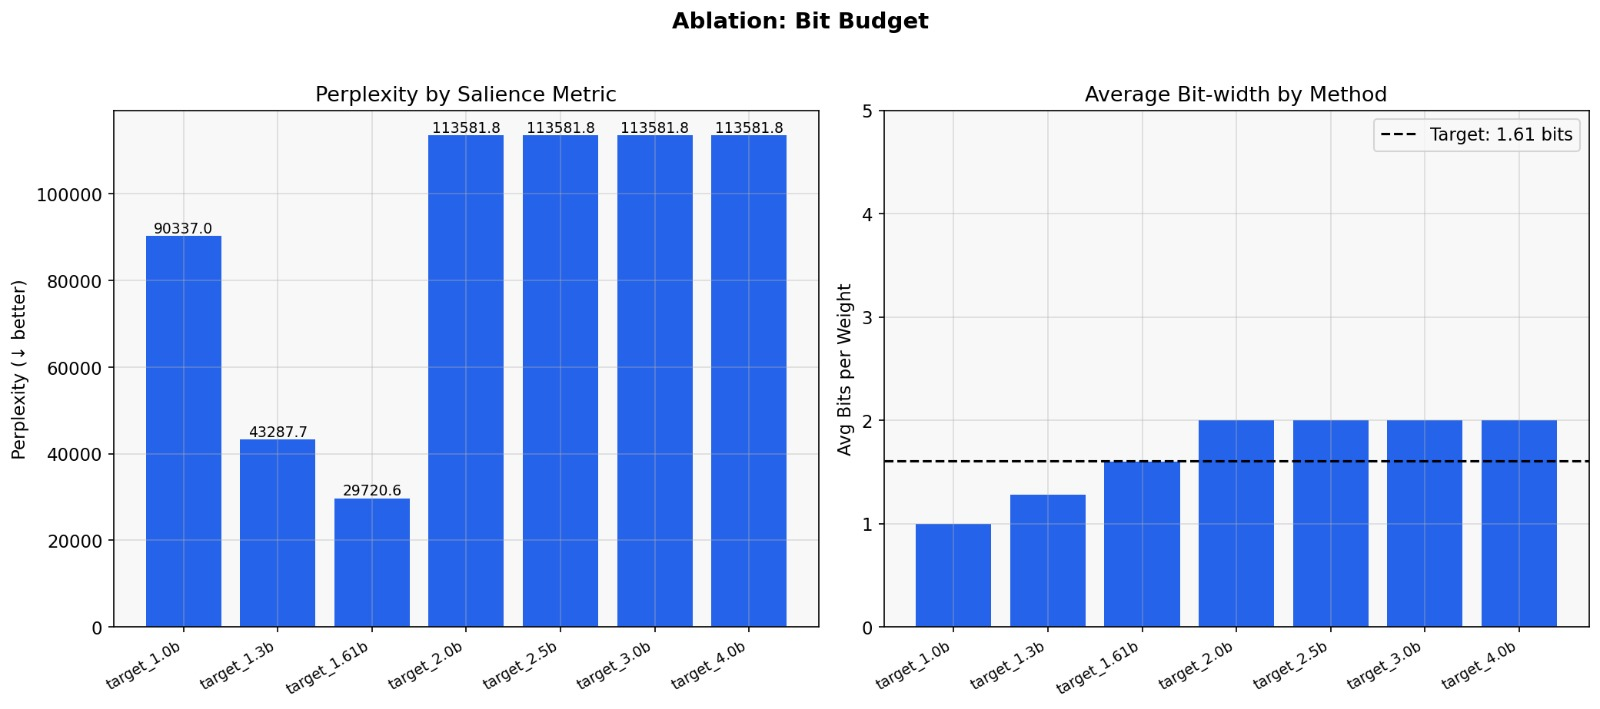
\includegraphics[width=0.92\textwidth]{figures/ablation_bit_budget.jpeg}
\caption{Ablation~3: bit-budget sweep on LLaMA-3.2-1B with default ensemble weights.
Targets~$\geq 2.0$~b collapse to identical 113{,}582~PPL because the allocator's 4-bit tier
did not activate (see Section~\ref{sec:limits}); 1.61~b is the empirical optimum.}
\end{figure}

\section{Per-Ablation Plot Gallery}
\label{app:plots}

\begin{figure}[ht!]
\centering
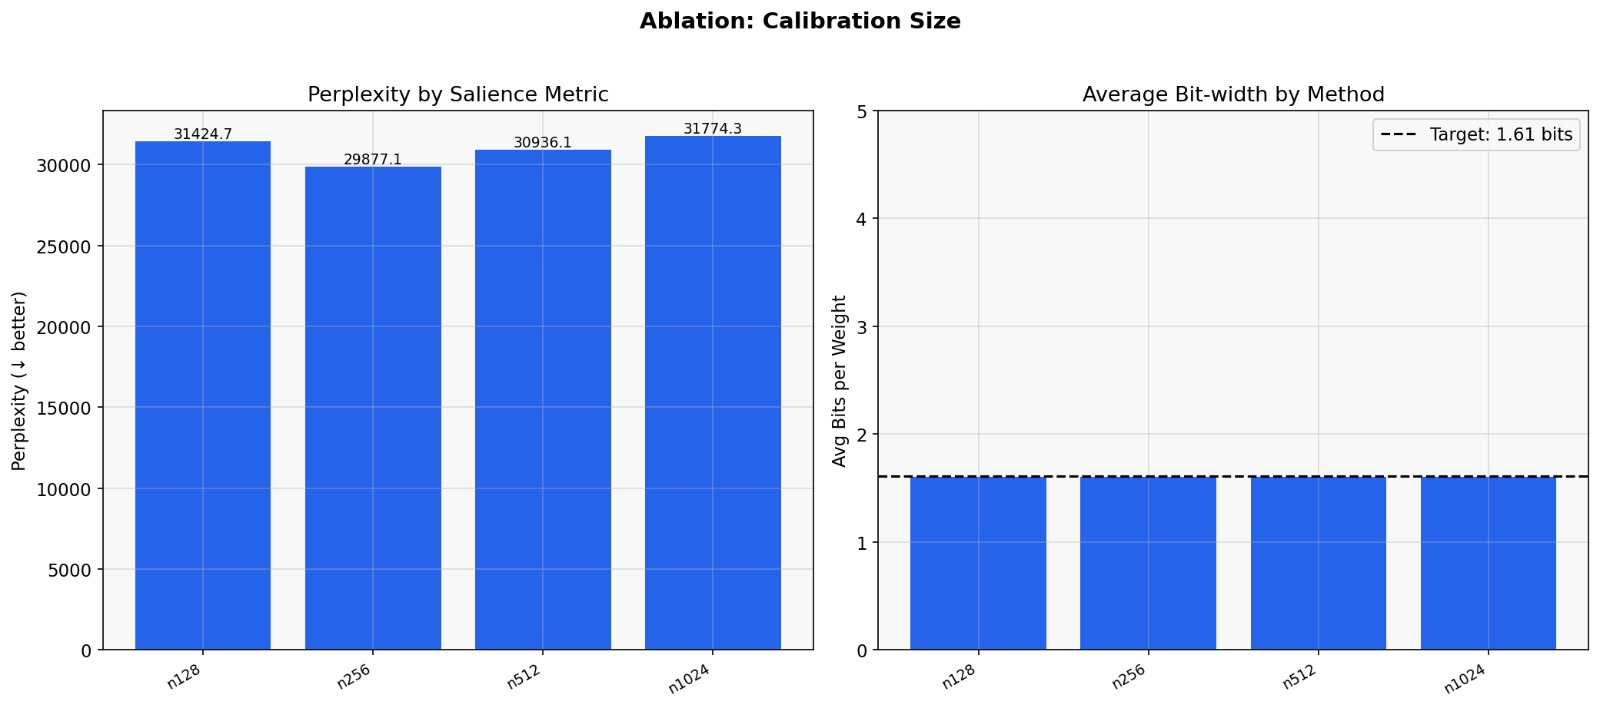
\includegraphics[width=0.66\textwidth]{figures/ablation_calibration_size.jpeg}
\caption{Ablation~4: calibration set size (LLaMA-1B, 1.61~b).
Salience saturates at $N{=}256$.}
\end{figure}

\begin{figure}[ht!]
\centering
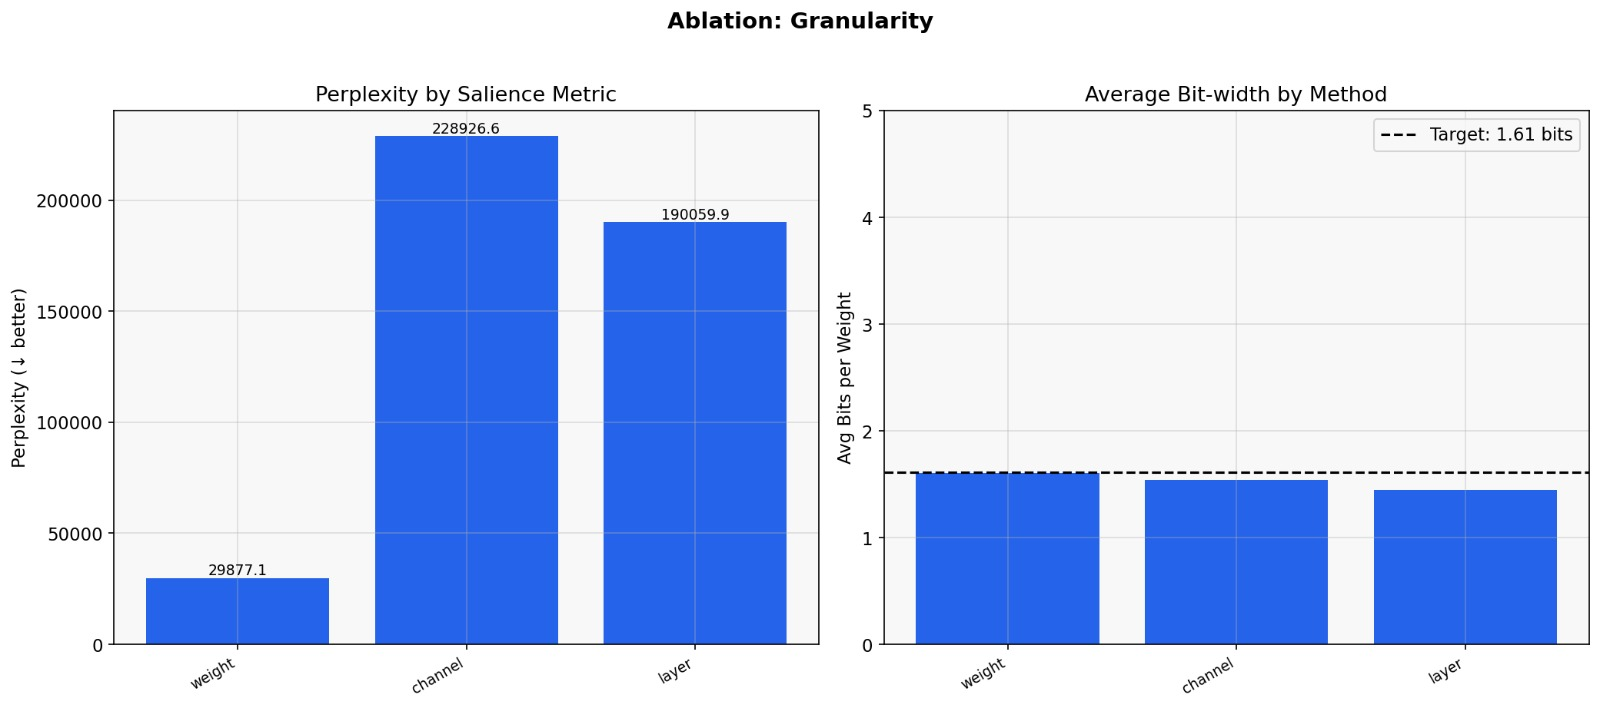
\includegraphics[width=0.66\textwidth]{figures/ablation_granularity.jpeg}
\caption{Ablation~5: granularity (LLaMA-1B, 1.61~b target).
Coarser granularities also undershoot the bit budget.}
\end{figure}

\begin{figure}[ht!]
\centering
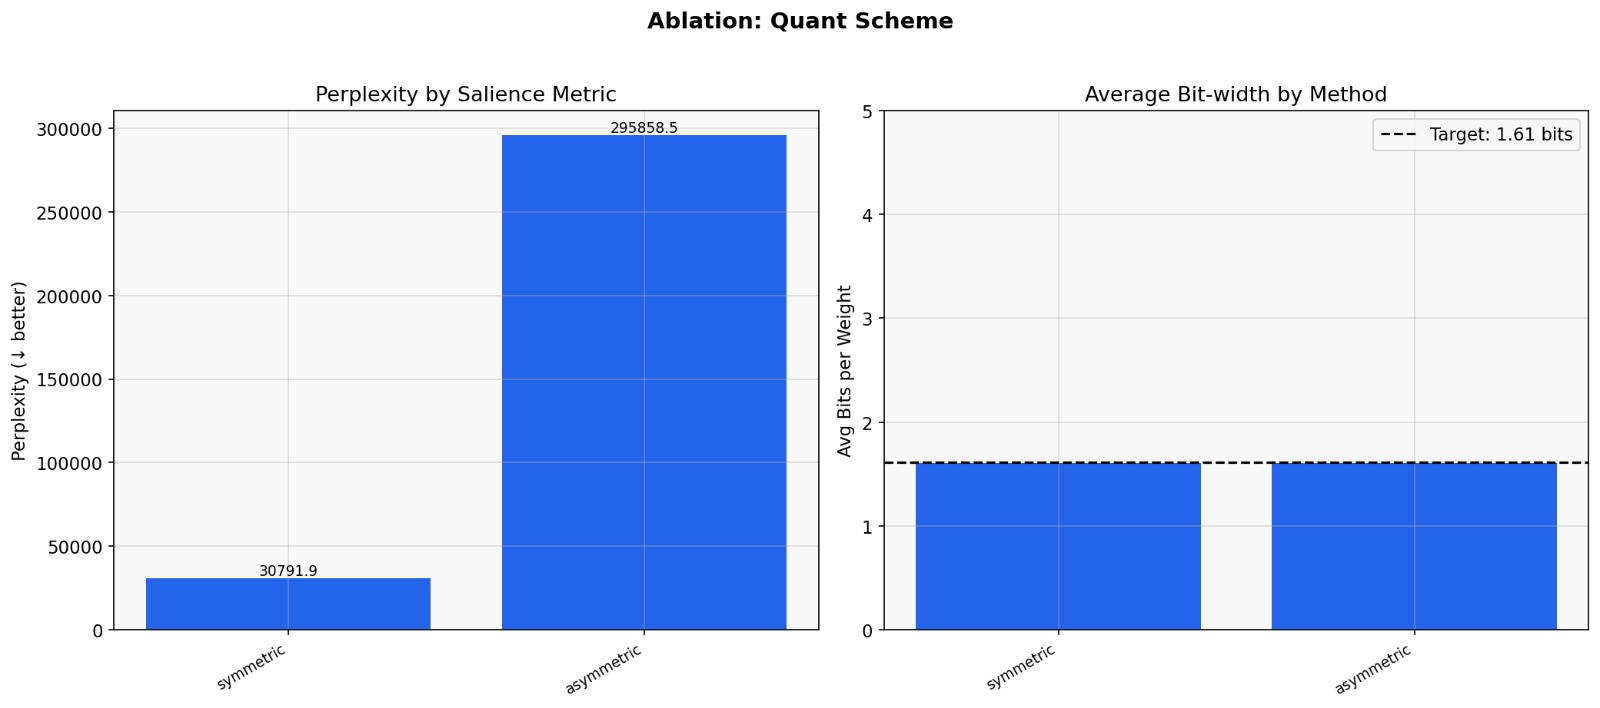
\includegraphics[width=0.66\textwidth]{figures/ablation_quant_scheme.jpeg}
\caption{Ablation~6: quantization scheme (LLaMA-1B, 1.61~b).
Symmetric is $9.6\times$ better than asymmetric on LLaMA; the deployed config should be
updated.}
\end{figure}

\begin{figure}[ht!]
\centering
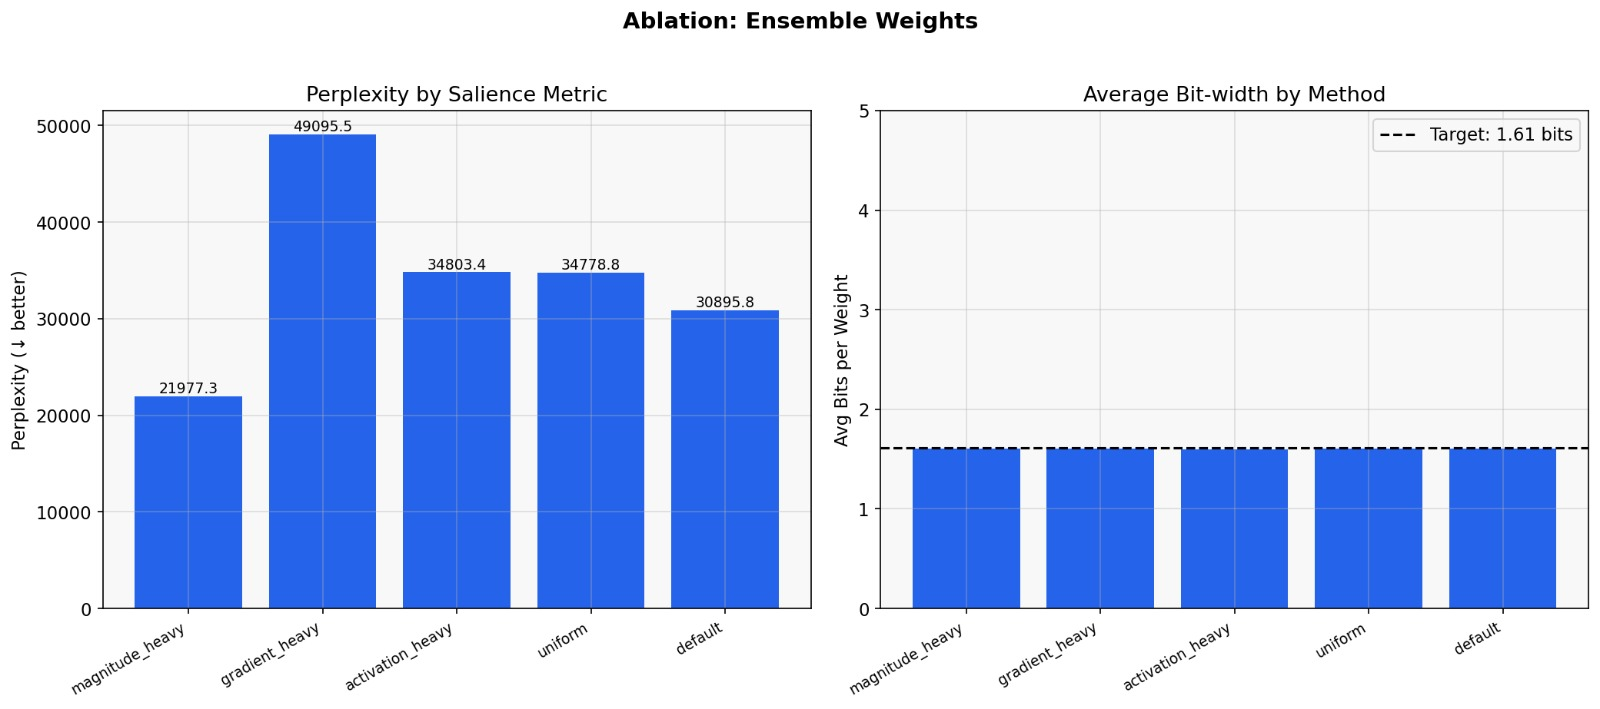
\includegraphics[width=0.66\textwidth]{figures/ablation_ensemble_weights.jpeg}
\caption{Ablation~7: ensemble weights (LLaMA-1B, 1.61~b).
Magnitude-heavy outperforms the gradient/Hessian-heavy default.}
\end{figure}

\section{Implementation Notes}
\label{app:impl}

\paragraph{Block size.}
GPT-2 and LLaMA pipelines both use \texttt{block\_size}=32; smaller blocks yield more
per-block scales (small overhead) at substantially better PPL.

\paragraph{Weight tying.}
GPT-2 shares the embedding (\texttt{wte}) with the output projection (\texttt{lm\_head})
via a data pointer alias.
Quantizing the tied head silently corrupts token embeddings ($\text{PPL} > 10^{11}$);
we detect and skip tied parameters via \texttt{data\_ptr()} comparison.

\paragraph{Architecture-specific behavior.}
GPT-2 uses \texttt{Conv1D} (shape \texttt{[in, out]}) rather than \texttt{nn.Linear}
(\texttt{[out, in]}); this required special handling in activation hook registration and
mixed-precision group extraction.
LLaMA uses \texttt{nn.Linear}; the codebase handles both via a 2D weight scan fallback.

\paragraph{Random seeds.}
All experiments use seed~42 unless noted; ablation runs are re-seeded per configuration.

\end{document}
